\documentclass[a4paper 14pt]{article}
\usepackage[hyperref]{ctex}

%%===================通用package===================
\usepackage{pdfpages}
\usepackage{ulem}
\usepackage{multirow,pgfplots,graphicx}
\usepackage{amssymb,amsfonts,amsthm,amsmath,bm,microtype}
\usepackage{indentfirst}
\usepackage{graphicx}
\usepackage{subfigure}
\usepackage{wrapfig}
\usepackage{enumerate}
\usepackage{abstract}
\usepackage{lastpage}                                           
\usepackage{layout} 
\usepackage{setspace}%行距设置
\usepackage[section]{placeins}%避免浮动体跨过 \section 等章节标题,可以在章节标题前,强制输出上一章节中尚未输出的浮动体。
\usepackage{bm}%给希腊字母加粗,格式为$\bm{\gamma}$


%======================自定义命令====================================
\newcommand{\pa}{\parallel}%平行符号
\newcommand{\vep}{\varepsilon}%varepsilon
\newcommand{\vp}{\varphi}%varphi
\newcommand{\f}{\frac{1}{2}}%1/2
\newcommand{\p}{\partial}





%%===================中文字体设置===============================
\usepackage{fontspec}
\usepackage{xunicode}
\usepackage{xltxtra} 
\setCJKfamilyfont{SimHei}{simhei.ttf}
\newcommand*{\HT}{\CJKfamily{SimHei}}%黑体
\setCJKfamilyfont{ST}{simsun.ttc}
\newcommand*{\ST}{\CJKfamily{ST}} %宋体
\setCJKfamilyfont{KT}{simkai.ttf}
\newcommand*{\KT}{\CJKfamily{KT}} %楷体
\setCJKfamilyfont{SH}{STZHONGS.TTF}
\newcommand*{\SH}{\CJKfamily{SH}} %华文中宋字体作为宋体加粗使用,格式为{\SH text}


%%%=================定义中文字体大小(字号对照表)=================================  
\newcommand{\chuhao}{\fontsize{42pt}{\baselineskip}\selectfont}     %初号  
\newcommand{\xiaochuhao}{\fontsize{36pt}{\baselineskip}\selectfont} %小初号  
\newcommand{\yihao}{\fontsize{28pt}{\baselineskip}\selectfont}      %一号  
\newcommand{\erhao}{\fontsize{21pt}{\baselineskip}\selectfont}      %二号  
\newcommand{\xiaoerhao}{\fontsize{18pt}{\baselineskip}\selectfont}  %小二号  
\newcommand{\sanhao}{\fontsize{15.75pt}{\baselineskip}\selectfont}  %三号  
\newcommand{\sihao}{\fontsize{14pt}{\baselineskip}\selectfont}%     四号  
\newcommand{\xiaosihao}{\fontsize{12pt}{\baselineskip}\selectfont}  %小四号  
\newcommand{\wuhao}{\fontsize{10.5pt}{\baselineskip}\selectfont}    %五号  
\newcommand{\xiaowuhao}{\fontsize{9pt}{\baselineskip}\selectfont}   %小五号  
\newcommand{\liuhao}{\fontsize{7.875pt}{\baselineskip}\selectfont}  %六号  
\newcommand{\qihao}{\fontsize{5.25pt}{\baselineskip}\selectfont}    %七号
\setCJKmainfont{SimSun}%设置全局主字体为宋体
\setmainfont{Times New Roman}



%==================================定义页面边距===================================================
\renewcommand{\baselinestretch}{1.2}  %1.2倍行距
\usepackage{geometry}
\geometry{left=2.8cm,right=2.8cm,top=2.54cm,bottom=2.54cm}



%==================================定义标题样式===================================================

\usepackage{titlesec}
\titleformat{\part}%设置part的样式
{\raggedright\sihao\HT}%左对齐,4号字,黑体
{\text{\bf Chapter}\quad\thepart \quad}
{0pt}%sep label和title之间的水平距离
{}%标题前没有内容
\titleformat{\section}%设置section的样式
{\raggedright\sihao\HT}%左对齐,4号字,黑体
{\thesection \quad}
{0pt}%sep label和title之间的水平距离
{}%标题前没有内容

\titleformat{\subsection}%设置subsection的样式
{\raggedright\sihao\HT}%左对齐,4号字,黑体
{\thesubsection \quad}
{0pt}%sep label和title之间的水平距离
{}%标题前没有内容

\titleformat{\subsubsection}%设置subsubsection的样式
{\raggedright\sihao\HT}%左对齐,4号字,黑体
{\thesubsubsection \quad}
{0pt}%sep label和title之间的水平距离
{}%标题前没有内容


%==================================目录格式设置===================================================

\usepackage{titletoc}

\titlecontents{part}[6mm]%标签距离页面左边距
{\fontsize{14pt}{20pt}\selectfont \HT} %四号-14pt,黑体
{\contentslabel{2.5em}}%标签距离目录内容距离
{}
{\titlerule*{.}\contentspage}

\titlecontents{section}[22mm]%标签距离页面左边距
{\fontsize{14pt}{20pt}\selectfont \HT} %四号-14pt,黑体
{\contentslabel{2.5em}}%标签距离目录内容距离
{}
{\titlerule*{.}\contentspage}

\titlecontents{subsection}[32mm]%标签距离页面左边距
{\fontsize{12pt}{20pt}\selectfont \ST }%小四号-12pt,宋体
{\contentslabel{3.3em}}  %标签距离目录内容距离
{}
{\titlerule*{.}\contentspage}

\titlecontents{subsubsection}[44mm]%标签距离页面左边距
{\fontsize{12pt}{20pt}\selectfont \ST }
{\contentslabel{4.1em}}  %标签距离目录内容距离
{}
{\titlerule*{.}\contentspage}
\renewcommand{\contentsname}{\hspace*{\fill}{\sanhao 目}\quad{\sanhao 录}\hspace*{\fill}}%设置“目录”居中和四号字加粗


%==================================页眉页脚设置==================================
\usepackage{fancyhdr}%页眉页脚
\pagestyle{fancy}

\fancyhead{}
\fancyhead[RO]{\small \rightmark}%\rightmark代替当前section名,\leftmark代替当前chapter名。
\fancyhead[RO,LE]{\small \rightmark}
\fancyfoot[C]{\wuhao \thepage}
\fancyfoot[RO,LE]{\textcolor[RGB]{144,144,144}{\emph{Ordered by Chihchao Mao}}}
\renewcommand{\headrulewidth}{0pt}%改为0pt即可去掉页眉下面的横线
\renewcommand{\footrulewidth}{0pt}%改为0pt即可去掉页脚上面的横线


%==========================公式、图片、表格按章节编号设定========================
\makeatletter
\@addtoreset{equation}{section}
\makeatother
\renewcommand{\theequation}{\arabic{section}.\arabic{equation}}%公式按章节编号
\numberwithin{figure}{section} %图片编号小号随section清零
\numberwithin{table}{section} %表格编号小号随section清零
\renewcommand{\thefigure}{\arabic{section}-\arabic{figure}}%图片按章节编号
\renewcommand{\thetable}{\arabic{section}.\arabic{table}}%表格按章节编号


%================================标题作者日期=================================
\title{Common}
\author{Chihchao Mao}
\date{}%日期,{}为缺省


\begin{document}
	\maketitle
	\pagenumbering{arabic}
	\xiaosihao

This is a common XeLaTex Model for sharing. And here are some useful example below.


\section{Mathematical Expression}
\subsection{Cases}
	\begin{equation}
		f(x)=
			\begin{cases}
				y_1,a_3<x<a_4\\
				y_2,a_1<x<a_2
			\end{cases}
	\end{equation}

\subsection{Matrix}
	\begin{equation}
		\left[              
		\begin{array}{cc}   
			a & b \\  
			c & d \\  
		\end{array}
		\right]. 	
	\end{equation} 

\section{Table}
	\begin{table}[htbp]
		\centering
			\begin{tabular}{c|c|c|c}
			\hline
			 $A_0$ & $A_1$ & $A_2$ & $A_3$\\
			\hline
			1 & 5 & 9 & 13 \\
			2 & 6 & 10 & 14 \\
			3 & 7 & 11 & 15 \\
			4 & 8 & 12 &  16 \\
			\hline
			\end{tabular}
		\caption{Table Example}
	\end{table}	

\section{Figures}
/Latex Example/Latex Example/Latex Example/Latex Example/Latex Example/Latex Example/Latex Example/Latex Example/Latex Example/Latex Example/Latex Example/Latex Example/Latex Example/Latex Example/Latex Example/Latex Example/Latex Example/Latex Example/Latex Example/Latex Example/Latex Example
\begin{figure}[htbp]
	\centering
	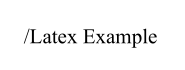
\includegraphics[width=0.2\textwidth]{figures//example.png}
	\caption{Example}
\end{figure}
/Latex Example/Latex Example/Latex Example/Latex Example/Latex Example/Latex Example/Latex Example/Latex Example/Latex Example/Latex Example/Latex Example/Latex Example/Latex Example/Latex Example/Latex Example/Latex Example/Latex Example/Latex Example/Latex Example/Latex Example/Latex Example/Latex Example/Latex Example/Latex Example/Latex Example/Latex Example/Latex Example/Latex Example/Latex Example/Latex Example/Latex Example/Latex Example/Latex Example/Latex Example/Latex Example/Latex Example/Latex Example/Latex Example/Latex Example/Latex Example/Latex Example/Latex Example/Latex Example/Latex Example/Latex Example/Latex Example/Latex Example/Latex Example/Latex Example/Latex Example/Latex Example/Latex Example/Latex Example/Latex Example/Latex Example/Latex Example/Latex Example/Latex Example/Latex Example/Latex Example/Latex Example/Latex Example/Latex \begin{wrapfigure}{r}{0.5\textwidth}
	\vspace{-20pt}
	\begin{center}
		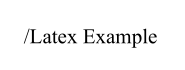
\includegraphics[width=0.3\textwidth]{figures//example.png}
	\end{center}
	\vspace{-20pt}
	\caption{Example 2()}
	\vspace{-10pt}
\end{wrapfigure}Example/Latex Example/Latex Example/Latex Example/Latex Example/Latex Example/Latex Example/Latex Example/Latex Example/Latex Example/Latex Example/Latex Example/Latex Example/Latex Example/Latex Example/Latex Example/Latex Example/Latex Example/Latex Example/Latex Example/Latex Example/Latex Example/Latex Example/Latex Example/Latex Example/Latex Example
\begin{figure}[htbp]
	\centering
	\subfigure[]{
		\begin{minipage}{7cm}
			\centering
			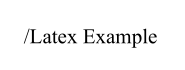
\includegraphics[width=0.3\textwidth]{figures//example.png}
	\end{minipage}}
	\subfigure[]{
		\begin{minipage}{7cm}
			\centering
			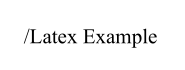
\includegraphics[width=0.3\textwidth]{figures//example.png}
	\end{minipage}}	
	\caption{Two figures}
\end{figure}

\end{document}